\documentclass[twoside]{book}

% Packages required by doxygen
\usepackage{fixltx2e}
\usepackage{calc}
\usepackage{doxygen}
\usepackage[export]{adjustbox} % also loads graphicx
\usepackage{graphicx}
\usepackage[utf8]{inputenc}
\usepackage{makeidx}
\usepackage{multicol}
\usepackage{multirow}
\PassOptionsToPackage{warn}{textcomp}
\usepackage{textcomp}
\usepackage[nointegrals]{wasysym}
\usepackage[table]{xcolor}

% Font selection
\usepackage[T1]{fontenc}
\usepackage[scaled=.90]{helvet}
\usepackage{courier}
\usepackage{amssymb}
\usepackage{sectsty}
\renewcommand{\familydefault}{\sfdefault}
\allsectionsfont{%
  \fontseries{bc}\selectfont%
  \color{darkgray}%
}
\renewcommand{\DoxyLabelFont}{%
  \fontseries{bc}\selectfont%
  \color{darkgray}%
}
\newcommand{\+}{\discretionary{\mbox{\scriptsize$\hookleftarrow$}}{}{}}

% Page & text layout
\usepackage{geometry}
\geometry{%
  a4paper,%
  top=2.5cm,%
  bottom=2.5cm,%
  left=2.5cm,%
  right=2.5cm%
}
\tolerance=750
\hfuzz=15pt
\hbadness=750
\setlength{\emergencystretch}{15pt}
\setlength{\parindent}{0cm}
\setlength{\parskip}{3ex plus 2ex minus 2ex}
\makeatletter
\renewcommand{\paragraph}{%
  \@startsection{paragraph}{4}{0ex}{-1.0ex}{1.0ex}{%
    \normalfont\normalsize\bfseries\SS@parafont%
  }%
}
\renewcommand{\subparagraph}{%
  \@startsection{subparagraph}{5}{0ex}{-1.0ex}{1.0ex}{%
    \normalfont\normalsize\bfseries\SS@subparafont%
  }%
}
\makeatother

% Headers & footers
\usepackage{fancyhdr}
\pagestyle{fancyplain}
\fancyhead[LE]{\fancyplain{}{\bfseries\thepage}}
\fancyhead[CE]{\fancyplain{}{}}
\fancyhead[RE]{\fancyplain{}{\bfseries\leftmark}}
\fancyhead[LO]{\fancyplain{}{\bfseries\rightmark}}
\fancyhead[CO]{\fancyplain{}{}}
\fancyhead[RO]{\fancyplain{}{\bfseries\thepage}}
\fancyfoot[LE]{\fancyplain{}{}}
\fancyfoot[CE]{\fancyplain{}{}}
\fancyfoot[RE]{\fancyplain{}{\bfseries\scriptsize Generated by Doxygen }}
\fancyfoot[LO]{\fancyplain{}{\bfseries\scriptsize Generated by Doxygen }}
\fancyfoot[CO]{\fancyplain{}{}}
\fancyfoot[RO]{\fancyplain{}{}}
\renewcommand{\footrulewidth}{0.4pt}
\renewcommand{\chaptermark}[1]{%
  \markboth{#1}{}%
}
\renewcommand{\sectionmark}[1]{%
  \markright{\thesection\ #1}%
}

% Indices & bibliography
\usepackage{natbib}
\usepackage[titles]{tocloft}
\setcounter{tocdepth}{3}
\setcounter{secnumdepth}{5}
\makeindex

% Hyperlinks (required, but should be loaded last)
\usepackage{ifpdf}
\ifpdf
  \usepackage[pdftex,pagebackref=true]{hyperref}
\else
  \usepackage[ps2pdf,pagebackref=true]{hyperref}
\fi
\hypersetup{%
  colorlinks=true,%
  linkcolor=blue,%
  citecolor=blue,%
  unicode%
}

% Custom commands
\newcommand{\clearemptydoublepage}{%
  \newpage{\pagestyle{empty}\cleardoublepage}%
}

\usepackage{caption}
\captionsetup{labelsep=space,justification=centering,font={bf},singlelinecheck=off,skip=4pt,position=top}

%===== C O N T E N T S =====

\begin{document}

% Titlepage & ToC
\hypersetup{pageanchor=false,
             bookmarksnumbered=true,
             pdfencoding=unicode
            }
\pagenumbering{alph}
\begin{titlepage}
\vspace*{7cm}
\begin{center}%
{\Large Ray\+\_\+tracing }\\
\vspace*{1cm}
{\large Generated by Doxygen 1.8.14}\\
\end{center}
\end{titlepage}
\clearemptydoublepage
\pagenumbering{roman}
\tableofcontents
\clearemptydoublepage
\pagenumbering{arabic}
\hypersetup{pageanchor=true}

%--- Begin generated contents ---
\chapter{Hierarchical Index}
\section{Class Hierarchy}
This inheritance list is sorted roughly, but not completely, alphabetically\+:\begin{DoxyCompactList}
\item \contentsline{section}{Camera}{\pageref{class_camera}}{}
\item \contentsline{section}{Material}{\pageref{class_material}}{}
\item \contentsline{section}{Ray3f}{\pageref{class_ray3f}}{}
\item \contentsline{section}{Scene}{\pageref{class_scene}}{}
\item \contentsline{section}{Shape}{\pageref{class_shape}}{}
\begin{DoxyCompactList}
\item \contentsline{section}{Cube\+Quad}{\pageref{class_cube_quad}}{}
\item \contentsline{section}{Sphere}{\pageref{class_sphere}}{}
\end{DoxyCompactList}
\item \contentsline{section}{Vector3f}{\pageref{class_vector3f}}{}
\end{DoxyCompactList}

\chapter{Class Index}
\section{Class List}
Here are the classes, structs, unions and interfaces with brief descriptions\+:\begin{DoxyCompactList}
\item\contentsline{section}{\mbox{\hyperlink{class_camera}{Camera}} }{\pageref{class_camera}}{}
\item\contentsline{section}{\mbox{\hyperlink{class_cube_quad}{Cube\+Quad}} }{\pageref{class_cube_quad}}{}
\item\contentsline{section}{\mbox{\hyperlink{class_material}{Material}} }{\pageref{class_material}}{}
\item\contentsline{section}{\mbox{\hyperlink{class_ray3f}{Ray3f}} }{\pageref{class_ray3f}}{}
\item\contentsline{section}{\mbox{\hyperlink{class_scene}{Scene}} }{\pageref{class_scene}}{}
\item\contentsline{section}{\mbox{\hyperlink{class_shape}{Shape}} }{\pageref{class_shape}}{}
\item\contentsline{section}{\mbox{\hyperlink{class_sphere}{Sphere}} }{\pageref{class_sphere}}{}
\item\contentsline{section}{\mbox{\hyperlink{class_vector3f}{Vector3f}} }{\pageref{class_vector3f}}{}
\end{DoxyCompactList}

\chapter{Class Documentation}
\hypertarget{class_camera}{}\section{Camera Class Reference}
\label{class_camera}\index{Camera@{Camera}}
\subsection*{Public Member Functions}
\begin{DoxyCompactItemize}
\item 
\mbox{\hyperlink{class_camera_a7992e90d78d3ad86ad83ba4a4879fc48}{Camera}} (\mbox{\hyperlink{class_vector3f}{Vector3f}} position, \mbox{\hyperlink{class_vector3f}{Vector3f}} direction)
\item 
\mbox{\hyperlink{class_vector3f}{Vector3f}} \mbox{\hyperlink{class_camera_a4e257bcf641d333ce77bac775792a9c3}{get\+Position}} () const
\item 
\mbox{\hyperlink{class_vector3f}{Vector3f}} \mbox{\hyperlink{class_camera_ad28f4c7b4ee77d2837c20beeb94d00c2}{get\+Direction}} () const
\end{DoxyCompactItemize}


\subsection{Constructor \& Destructor Documentation}
\mbox{\Hypertarget{class_camera_a7992e90d78d3ad86ad83ba4a4879fc48}\label{class_camera_a7992e90d78d3ad86ad83ba4a4879fc48}} 
\index{Camera@{Camera}!Camera@{Camera}}
\index{Camera@{Camera}!Camera@{Camera}}
\subsubsection{\texorpdfstring{Camera()}{Camera()}}
{\footnotesize\ttfamily Camera\+::\+Camera (\begin{DoxyParamCaption}\item[{\mbox{\hyperlink{class_vector3f}{Vector3f}}}]{position,  }\item[{\mbox{\hyperlink{class_vector3f}{Vector3f}}}]{direction }\end{DoxyParamCaption})}

\begin{DoxyReturn}{Returns}
\mbox{\hyperlink{class_camera}{Camera}} \+: New instance of \mbox{\hyperlink{class_camera}{Camera}} 
\end{DoxyReturn}


\subsection{Member Function Documentation}
\mbox{\Hypertarget{class_camera_ad28f4c7b4ee77d2837c20beeb94d00c2}\label{class_camera_ad28f4c7b4ee77d2837c20beeb94d00c2}} 
\index{Camera@{Camera}!get\+Direction@{get\+Direction}}
\index{get\+Direction@{get\+Direction}!Camera@{Camera}}
\subsubsection{\texorpdfstring{get\+Direction()}{getDirection()}}
{\footnotesize\ttfamily \mbox{\hyperlink{class_vector3f}{Vector3f}} Camera\+::get\+Direction (\begin{DoxyParamCaption}{ }\end{DoxyParamCaption}) const\hspace{0.3cm}{\ttfamily [inline]}}

\begin{DoxyReturn}{Returns}
\mbox{\hyperlink{class_vector3f}{Vector3f}} \+: the direction of the camera 
\end{DoxyReturn}
\mbox{\Hypertarget{class_camera_a4e257bcf641d333ce77bac775792a9c3}\label{class_camera_a4e257bcf641d333ce77bac775792a9c3}} 
\index{Camera@{Camera}!get\+Position@{get\+Position}}
\index{get\+Position@{get\+Position}!Camera@{Camera}}
\subsubsection{\texorpdfstring{get\+Position()}{getPosition()}}
{\footnotesize\ttfamily \mbox{\hyperlink{class_vector3f}{Vector3f}} Camera\+::get\+Position (\begin{DoxyParamCaption}{ }\end{DoxyParamCaption}) const\hspace{0.3cm}{\ttfamily [inline]}}

\begin{DoxyReturn}{Returns}
\mbox{\hyperlink{class_vector3f}{Vector3f}} \+: the position of the camera 
\end{DoxyReturn}


The documentation for this class was generated from the following files\+:\begin{DoxyCompactItemize}
\item 
Camera.\+h\item 
Camera.\+cpp\end{DoxyCompactItemize}

\hypertarget{class_cube_quad}{}\section{Cube\+Quad Class Reference}
\label{class_cube_quad}\index{Cube\+Quad@{Cube\+Quad}}
Inheritance diagram for Cube\+Quad\+:\begin{figure}[H]
\begin{center}
\leavevmode
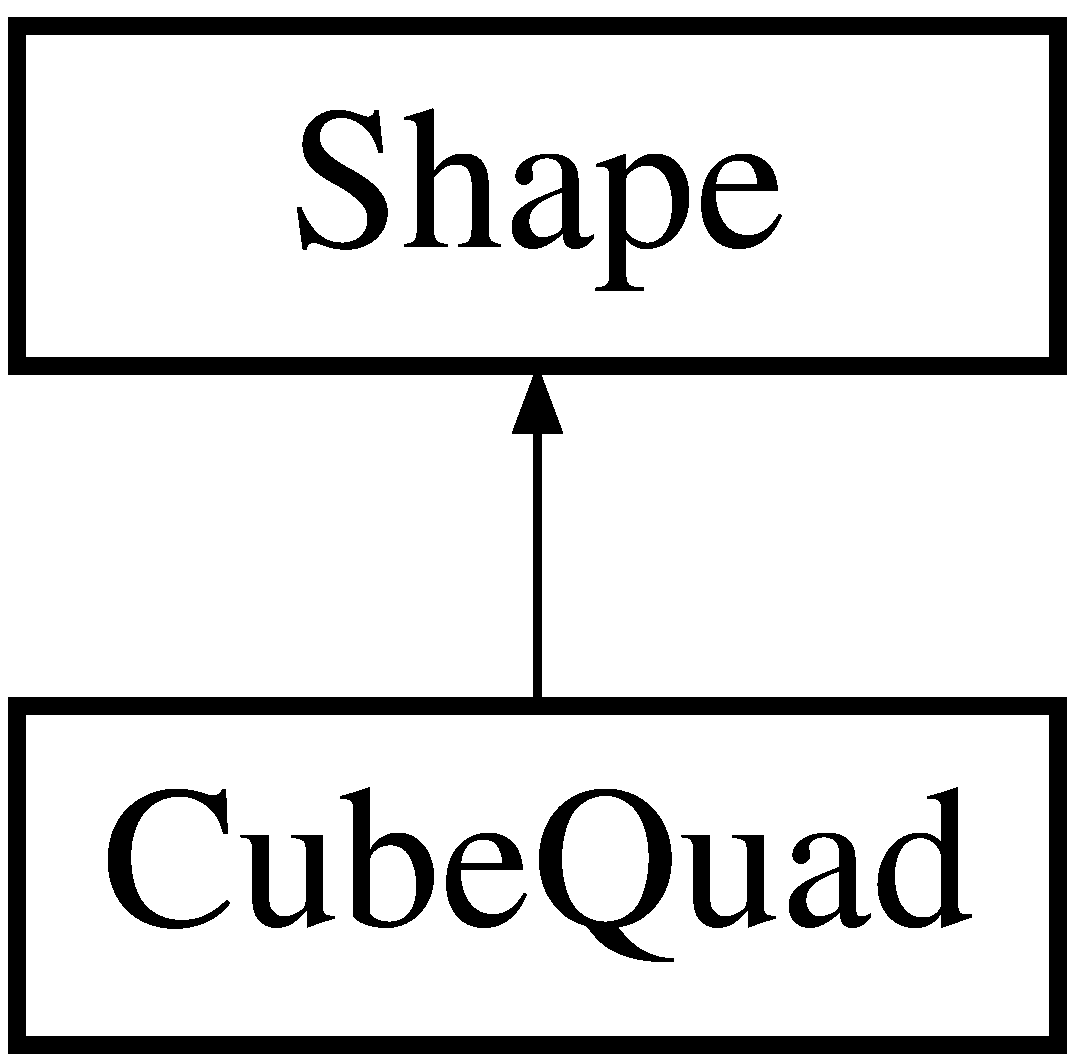
\includegraphics[height=2.000000cm]{class_cube_quad}
\end{center}
\end{figure}
\subsection*{Public Member Functions}
\begin{DoxyCompactItemize}
\item 
\mbox{\hyperlink{class_cube_quad_a3fa4c62ac49699d72d1a8c8fdca2f2cb}{Cube\+Quad}} (\mbox{\hyperlink{class_material}{Material}} m, \mbox{\hyperlink{class_vector3f}{Vector3f}} origin, \mbox{\hyperlink{class_vector3f}{Vector3f}} width, \mbox{\hyperlink{class_vector3f}{Vector3f}} height)
\item 
\mbox{\hyperlink{class_vector3f}{Vector3f}} \mbox{\hyperlink{class_cube_quad_abe8372c7f59cd9ff9a5a668fcd437a76}{get\+Origin}} () const
\item 
\mbox{\hyperlink{class_vector3f}{Vector3f}} \mbox{\hyperlink{class_cube_quad_a7229846a07dc9f641d16a488da740a49}{get\+Width}} () const
\item 
\mbox{\hyperlink{class_vector3f}{Vector3f}} \mbox{\hyperlink{class_cube_quad_adfb45d0ba7d9fce02b6ee82a7872262f}{get\+Height}} () const
\item 
virtual bool \mbox{\hyperlink{class_cube_quad_a8d55228ceeed7ce319bc6d8fe8f6b67f}{is\+\_\+hit}} (\mbox{\hyperlink{class_ray3f}{Ray3f}} \&ray)
\begin{DoxyCompactList}\small\item\em Find if there\textquotesingle{}s an intersection between an object and a ray. \end{DoxyCompactList}\item 
virtual \mbox{\hyperlink{class_ray3f}{Ray3f}} \mbox{\hyperlink{class_cube_quad_a18ef5943f0cfd8b9b72950211691314a}{reflect}} (\mbox{\hyperlink{class_ray3f}{Ray3f}} ray)
\begin{DoxyCompactList}\small\item\em Give the reflection ray of another ray that hit an object. \end{DoxyCompactList}\item 
virtual double \mbox{\hyperlink{class_cube_quad_a3b51f8216f2ba340174edb542af33c0a}{Intersection}} (\mbox{\hyperlink{class_ray3f}{Ray3f}} ray)
\begin{DoxyCompactList}\small\item\em Find the intersection position between an object and a ray. \end{DoxyCompactList}\item 
virtual \mbox{\hyperlink{class_vector3f}{Vector3f}} \mbox{\hyperlink{class_cube_quad_aba1f984ce9580e2e430ace0137a0f249}{get\+Normal}} (\mbox{\hyperlink{class_vector3f}{Vector3f}} position)
\begin{DoxyCompactList}\small\item\em Find the normal vector of an object. \end{DoxyCompactList}\end{DoxyCompactItemize}
\subsection*{Additional Inherited Members}


\subsection{Constructor \& Destructor Documentation}
\mbox{\Hypertarget{class_cube_quad_a3fa4c62ac49699d72d1a8c8fdca2f2cb}\label{class_cube_quad_a3fa4c62ac49699d72d1a8c8fdca2f2cb}} 
\index{Cube\+Quad@{Cube\+Quad}!Cube\+Quad@{Cube\+Quad}}
\index{Cube\+Quad@{Cube\+Quad}!Cube\+Quad@{Cube\+Quad}}
\subsubsection{\texorpdfstring{Cube\+Quad()}{CubeQuad()}}
{\footnotesize\ttfamily Cube\+Quad\+::\+Cube\+Quad (\begin{DoxyParamCaption}\item[{\mbox{\hyperlink{class_material}{Material}}}]{m,  }\item[{\mbox{\hyperlink{class_vector3f}{Vector3f}}}]{origin,  }\item[{\mbox{\hyperlink{class_vector3f}{Vector3f}}}]{width,  }\item[{\mbox{\hyperlink{class_vector3f}{Vector3f}}}]{height }\end{DoxyParamCaption})}

\begin{DoxyReturn}{Returns}
\mbox{\hyperlink{class_cube_quad}{Cube\+Quad}} \+: New instance of \mbox{\hyperlink{class_cube_quad}{Cube\+Quad}} 
\end{DoxyReturn}


\subsection{Member Function Documentation}
\mbox{\Hypertarget{class_cube_quad_adfb45d0ba7d9fce02b6ee82a7872262f}\label{class_cube_quad_adfb45d0ba7d9fce02b6ee82a7872262f}} 
\index{Cube\+Quad@{Cube\+Quad}!get\+Height@{get\+Height}}
\index{get\+Height@{get\+Height}!Cube\+Quad@{Cube\+Quad}}
\subsubsection{\texorpdfstring{get\+Height()}{getHeight()}}
{\footnotesize\ttfamily \mbox{\hyperlink{class_vector3f}{Vector3f}} Cube\+Quad\+::get\+Height (\begin{DoxyParamCaption}{ }\end{DoxyParamCaption}) const\hspace{0.3cm}{\ttfamily [inline]}}

\begin{DoxyReturn}{Returns}
\mbox{\hyperlink{class_vector3f}{Vector3f}} \+: The Height of the Cube quad intercepted 
\end{DoxyReturn}
\mbox{\Hypertarget{class_cube_quad_aba1f984ce9580e2e430ace0137a0f249}\label{class_cube_quad_aba1f984ce9580e2e430ace0137a0f249}} 
\index{Cube\+Quad@{Cube\+Quad}!get\+Normal@{get\+Normal}}
\index{get\+Normal@{get\+Normal}!Cube\+Quad@{Cube\+Quad}}
\subsubsection{\texorpdfstring{get\+Normal()}{getNormal()}}
{\footnotesize\ttfamily virtual \mbox{\hyperlink{class_vector3f}{Vector3f}} Cube\+Quad\+::get\+Normal (\begin{DoxyParamCaption}\item[{\mbox{\hyperlink{class_vector3f}{Vector3f}}}]{position }\end{DoxyParamCaption})\hspace{0.3cm}{\ttfamily [inline]}, {\ttfamily [virtual]}}



Find the normal vector of an object. 

give the normal vector from a position 
\begin{DoxyParams}{Parameters}
{\em ray} & \mbox{\hyperlink{class_vector3f}{Vector3f}} \\
\hline
\end{DoxyParams}
\begin{DoxyReturn}{Returns}
\mbox{\hyperlink{class_vector3f}{Vector3f}}\+: the normal vector 
\end{DoxyReturn}


Implements \mbox{\hyperlink{class_shape_afba80076ff9eb95f7e7c4144e323590f}{Shape}}.

\mbox{\Hypertarget{class_cube_quad_abe8372c7f59cd9ff9a5a668fcd437a76}\label{class_cube_quad_abe8372c7f59cd9ff9a5a668fcd437a76}} 
\index{Cube\+Quad@{Cube\+Quad}!get\+Origin@{get\+Origin}}
\index{get\+Origin@{get\+Origin}!Cube\+Quad@{Cube\+Quad}}
\subsubsection{\texorpdfstring{get\+Origin()}{getOrigin()}}
{\footnotesize\ttfamily \mbox{\hyperlink{class_vector3f}{Vector3f}} Cube\+Quad\+::get\+Origin (\begin{DoxyParamCaption}{ }\end{DoxyParamCaption}) const\hspace{0.3cm}{\ttfamily [inline]}}

\begin{DoxyReturn}{Returns}
\mbox{\hyperlink{class_vector3f}{Vector3f}} \+: The origin of the cube quad 
\end{DoxyReturn}
\mbox{\Hypertarget{class_cube_quad_a7229846a07dc9f641d16a488da740a49}\label{class_cube_quad_a7229846a07dc9f641d16a488da740a49}} 
\index{Cube\+Quad@{Cube\+Quad}!get\+Width@{get\+Width}}
\index{get\+Width@{get\+Width}!Cube\+Quad@{Cube\+Quad}}
\subsubsection{\texorpdfstring{get\+Width()}{getWidth()}}
{\footnotesize\ttfamily \mbox{\hyperlink{class_vector3f}{Vector3f}} Cube\+Quad\+::get\+Width (\begin{DoxyParamCaption}{ }\end{DoxyParamCaption}) const\hspace{0.3cm}{\ttfamily [inline]}}

\begin{DoxyReturn}{Returns}
\mbox{\hyperlink{class_vector3f}{Vector3f}} \+: The Width of the Cube quad intercepted 
\end{DoxyReturn}
\mbox{\Hypertarget{class_cube_quad_a3b51f8216f2ba340174edb542af33c0a}\label{class_cube_quad_a3b51f8216f2ba340174edb542af33c0a}} 
\index{Cube\+Quad@{Cube\+Quad}!Intersection@{Intersection}}
\index{Intersection@{Intersection}!Cube\+Quad@{Cube\+Quad}}
\subsubsection{\texorpdfstring{Intersection()}{Intersection()}}
{\footnotesize\ttfamily double Cube\+Quad\+::\+Intersection (\begin{DoxyParamCaption}\item[{\mbox{\hyperlink{class_ray3f}{Ray3f}}}]{ray }\end{DoxyParamCaption})\hspace{0.3cm}{\ttfamily [virtual]}}



Find the intersection position between an object and a ray. 

give the intersection position if there\textquotesingle{}s an intersection return -\/1 if there\textquotesingle{}s no intersection 
\begin{DoxyParams}{Parameters}
{\em ray} & \mbox{\hyperlink{class_ray3f}{Ray3f}} \\
\hline
\end{DoxyParams}
\begin{DoxyReturn}{Returns}
double the distance from our ray origin to the point of intersection return -\/1 if there\textquotesingle{}s no intersection 
\end{DoxyReturn}


Implements \mbox{\hyperlink{class_shape_aae1d31ff6fb4237397bf11afd07d7e48}{Shape}}.

\mbox{\Hypertarget{class_cube_quad_a8d55228ceeed7ce319bc6d8fe8f6b67f}\label{class_cube_quad_a8d55228ceeed7ce319bc6d8fe8f6b67f}} 
\index{Cube\+Quad@{Cube\+Quad}!is\+\_\+hit@{is\+\_\+hit}}
\index{is\+\_\+hit@{is\+\_\+hit}!Cube\+Quad@{Cube\+Quad}}
\subsubsection{\texorpdfstring{is\+\_\+hit()}{is\_hit()}}
{\footnotesize\ttfamily bool Cube\+Quad\+::is\+\_\+hit (\begin{DoxyParamCaption}\item[{\mbox{\hyperlink{class_ray3f}{Ray3f}} \&}]{ray }\end{DoxyParamCaption})\hspace{0.3cm}{\ttfamily [virtual]}}



Find if there\textquotesingle{}s an intersection between an object and a ray. 

Find if there\textquotesingle{}s an intersection between an object and a ray and give intersect of ray3f\+: the value of the distance from ray\textquotesingle{}s origin to the point of intersection 
\begin{DoxyParams}{Parameters}
{\em ray} & \mbox{\hyperlink{class_ray3f}{Ray3f}} \\
\hline
\end{DoxyParams}
\begin{DoxyReturn}{Returns}
bool true if we have intersection 
\end{DoxyReturn}


Implements \mbox{\hyperlink{class_shape_ab443b81b74cfb1d248d23cc049da7ddd}{Shape}}.

\mbox{\Hypertarget{class_cube_quad_a18ef5943f0cfd8b9b72950211691314a}\label{class_cube_quad_a18ef5943f0cfd8b9b72950211691314a}} 
\index{Cube\+Quad@{Cube\+Quad}!reflect@{reflect}}
\index{reflect@{reflect}!Cube\+Quad@{Cube\+Quad}}
\subsubsection{\texorpdfstring{reflect()}{reflect()}}
{\footnotesize\ttfamily \mbox{\hyperlink{class_ray3f}{Ray3f}} Cube\+Quad\+::reflect (\begin{DoxyParamCaption}\item[{\mbox{\hyperlink{class_ray3f}{Ray3f}}}]{ray }\end{DoxyParamCaption})\hspace{0.3cm}{\ttfamily [virtual]}}



Give the reflection ray of another ray that hit an object. 

Give the reflection ray from the intersection position 
\begin{DoxyParams}{Parameters}
{\em ray} & \mbox{\hyperlink{class_ray3f}{Ray3f}} \\
\hline
\end{DoxyParams}
\begin{DoxyReturn}{Returns}
\mbox{\hyperlink{class_ray3f}{Ray3f}} \+: the reflected ray 
\end{DoxyReturn}


Implements \mbox{\hyperlink{class_shape_a7cc30a4c8e9564c51f6ab36554aa5cfc}{Shape}}.



The documentation for this class was generated from the following files\+:\begin{DoxyCompactItemize}
\item 
Cube\+Quad.\+h\item 
Cube\+Quad.\+cpp\end{DoxyCompactItemize}

\hypertarget{class_material}{}\section{Material Class Reference}
\label{class_material}\index{Material@{Material}}
\subsection*{Public Member Functions}
\begin{DoxyCompactItemize}
\item 
\mbox{\Hypertarget{class_material_ac8d5054ec7d38ef126591219a291999f}\label{class_material_ac8d5054ec7d38ef126591219a291999f}} 
{\bfseries Material} (float r, float g, float b, float s)
\item 
\mbox{\Hypertarget{class_material_aa0ebce03213f42c962d7c60fdab787a8}\label{class_material_aa0ebce03213f42c962d7c60fdab787a8}} 
float {\bfseries get\+Red} () const
\item 
\mbox{\Hypertarget{class_material_a4728d9ed4f2b6cd9c8f3096c68617f1b}\label{class_material_a4728d9ed4f2b6cd9c8f3096c68617f1b}} 
float {\bfseries get\+Green} () const
\item 
\mbox{\Hypertarget{class_material_aaac3b6e4848d1ced045d9790f89a8084}\label{class_material_aaac3b6e4848d1ced045d9790f89a8084}} 
float {\bfseries get\+Blue} () const
\item 
\mbox{\Hypertarget{class_material_ac65754d70c261b6065087fe3ce828872}\label{class_material_ac65754d70c261b6065087fe3ce828872}} 
float {\bfseries get\+Shininess} () const
\item 
\mbox{\Hypertarget{class_material_aa46b0d1d5557e3c86396aa9a65e7314e}\label{class_material_aa46b0d1d5557e3c86396aa9a65e7314e}} 
void {\bfseries set\+Red} (double R\+Value)
\item 
\mbox{\Hypertarget{class_material_a6bf2a435ca0ace3a9b119e4f9e351e29}\label{class_material_a6bf2a435ca0ace3a9b119e4f9e351e29}} 
void {\bfseries set\+Green} (double G\+Value)
\item 
\mbox{\Hypertarget{class_material_acb2577139eceee571387d00f6ef0ca57}\label{class_material_acb2577139eceee571387d00f6ef0ca57}} 
void {\bfseries set\+Blue} (double B\+Value)
\item 
\mbox{\Hypertarget{class_material_a029df1bddd0d3c53bf76ad7594d0248e}\label{class_material_a029df1bddd0d3c53bf76ad7594d0248e}} 
void {\bfseries set\+Shininess} (double S\+Value)
\item 
\mbox{\Hypertarget{class_material_a1e67e8e0621864187926176e1c08ad5c}\label{class_material_a1e67e8e0621864187926176e1c08ad5c}} 
\mbox{\hyperlink{class_material}{Material}} {\bfseries color\+Scalar} (double scalar)
\item 
\mbox{\Hypertarget{class_material_af35f9928158d8c75088fa1e43da0c5ae}\label{class_material_af35f9928158d8c75088fa1e43da0c5ae}} 
\mbox{\hyperlink{class_material}{Material}} {\bfseries color\+Add} (\mbox{\hyperlink{class_material}{Material}} color)
\item 
\mbox{\Hypertarget{class_material_a4c78a31f45d9512bd179e37c833c45b4}\label{class_material_a4c78a31f45d9512bd179e37c833c45b4}} 
\mbox{\hyperlink{class_material}{Material}} {\bfseries clip} ()
\end{DoxyCompactItemize}


The documentation for this class was generated from the following files\+:\begin{DoxyCompactItemize}
\item 
Material.\+h\item 
Material.\+cpp\end{DoxyCompactItemize}

\hypertarget{class_ray3f}{}\section{Ray3f Class Reference}
\label{class_ray3f}\index{Ray3f@{Ray3f}}
\subsection*{Public Member Functions}
\begin{DoxyCompactItemize}
\item 
\mbox{\Hypertarget{class_ray3f_a35d36b08a02e89335b1ad865e291f9c5}\label{class_ray3f_a35d36b08a02e89335b1ad865e291f9c5}} 
{\bfseries Ray3f} (\mbox{\hyperlink{class_vector3f}{Vector3f}} o, \mbox{\hyperlink{class_vector3f}{Vector3f}} d)
\item 
\mbox{\Hypertarget{class_ray3f_a33c510ea76f584e1cec55c8719b5c3b0}\label{class_ray3f_a33c510ea76f584e1cec55c8719b5c3b0}} 
\mbox{\hyperlink{class_vector3f}{Vector3f}} {\bfseries get\+Origin} () const
\item 
\mbox{\Hypertarget{class_ray3f_a1827ff88486d510b19e715af10e02935}\label{class_ray3f_a1827ff88486d510b19e715af10e02935}} 
\mbox{\hyperlink{class_vector3f}{Vector3f}} {\bfseries get\+Direction} () const
\item 
\mbox{\Hypertarget{class_ray3f_a7848c6486f8022c50eb1299422538129}\label{class_ray3f_a7848c6486f8022c50eb1299422538129}} 
double {\bfseries get\+Intersect} () const
\item 
\mbox{\Hypertarget{class_ray3f_adb303ff92b3a9b53b268592240c17833}\label{class_ray3f_adb303ff92b3a9b53b268592240c17833}} 
void {\bfseries set\+Origin} (\mbox{\hyperlink{class_vector3f}{Vector3f}} o)
\item 
\mbox{\Hypertarget{class_ray3f_a6b47185e8115983b249bc650124666b5}\label{class_ray3f_a6b47185e8115983b249bc650124666b5}} 
void {\bfseries set\+Direction} (\mbox{\hyperlink{class_vector3f}{Vector3f}} d)
\item 
\mbox{\Hypertarget{class_ray3f_a0878928f5323833c590c229ca058d027}\label{class_ray3f_a0878928f5323833c590c229ca058d027}} 
void {\bfseries set\+Intersect} (double i)
\end{DoxyCompactItemize}


The documentation for this class was generated from the following files\+:\begin{DoxyCompactItemize}
\item 
Ray3f.\+h\item 
Ray3f.\+cpp\end{DoxyCompactItemize}

\hypertarget{class_scene}{}\section{Scene Class Reference}
\label{class_scene}\index{Scene@{Scene}}
\subsection*{Public Member Functions}
\begin{DoxyCompactItemize}
\item 
\mbox{\Hypertarget{class_scene_aa722c9492bc4be765c6d8db718d52f1c}\label{class_scene_aa722c9492bc4be765c6d8db718d52f1c}} 
{\bfseries Scene} (\mbox{\hyperlink{class_camera}{Camera}} c, vector$<$ \mbox{\hyperlink{class_shape}{Shape}} $\ast$$>$ s, \mbox{\hyperlink{class_ray3f}{Ray3f}} r)
\item 
\mbox{\Hypertarget{class_scene_a6d0a3d4d98ee8c259109cdc14e7c5408}\label{class_scene_a6d0a3d4d98ee8c259109cdc14e7c5408}} 
\mbox{\hyperlink{class_camera}{Camera}} \mbox{\hyperlink{class_scene_a6d0a3d4d98ee8c259109cdc14e7c5408}{get\+Camera}} () const
\begin{DoxyCompactList}\small\item\em \mbox{\hyperlink{class_scene}{Scene}} getter. \end{DoxyCompactList}\item 
\mbox{\Hypertarget{class_scene_a04fdbafba14bf53aa5e6a4a492bc7a03}\label{class_scene_a04fdbafba14bf53aa5e6a4a492bc7a03}} 
vector$<$ \mbox{\hyperlink{class_shape}{Shape}} $\ast$ $>$ {\bfseries get\+Shapes} () const
\item 
\mbox{\Hypertarget{class_scene_a242762e0cf02fc62e90b8c2f65c833c5}\label{class_scene_a242762e0cf02fc62e90b8c2f65c833c5}} 
\mbox{\hyperlink{class_ray3f}{Ray3f}} {\bfseries get\+Source} () const
\item 
void \mbox{\hyperlink{class_scene_a8cc1bb60246aa6e3d8c41d1780d09f7e}{save}} (const char $\ast$filename, int w, int h, int dpi, \mbox{\hyperlink{class_material}{Material}} $\ast$couleur)
\item 
\mbox{\hyperlink{class_material}{Material}} \mbox{\hyperlink{class_scene_a9403e54c505999db1f88ebc722ebfab1}{get\+Color}} (\mbox{\hyperlink{class_ray3f}{Ray3f}} ray, int object\+\_\+index)
\begin{DoxyCompactList}\small\item\em Get the color of the intersection. \end{DoxyCompactList}\item 
void \mbox{\hyperlink{class_scene_a5fd03877e1c4e302c2229bc86d16a23a}{render}} (int width, int height, char $\ast$filename)
\begin{DoxyCompactList}\small\item\em Render the scene. \end{DoxyCompactList}\end{DoxyCompactItemize}


\subsection{Member Function Documentation}
\mbox{\Hypertarget{class_scene_a9403e54c505999db1f88ebc722ebfab1}\label{class_scene_a9403e54c505999db1f88ebc722ebfab1}} 
\index{Scene@{Scene}!get\+Color@{get\+Color}}
\index{get\+Color@{get\+Color}!Scene@{Scene}}
\subsubsection{\texorpdfstring{get\+Color()}{getColor()}}
{\footnotesize\ttfamily \mbox{\hyperlink{class_material}{Material}} Scene\+::get\+Color (\begin{DoxyParamCaption}\item[{\mbox{\hyperlink{class_ray3f}{Ray3f}}}]{ray,  }\item[{int}]{object\+\_\+index }\end{DoxyParamCaption})}



Get the color of the intersection. 


\begin{DoxyParams}{Parameters}
{\em \mbox{\hyperlink{class_ray3f}{Ray3f}}} & intercepted \\
\hline
{\em object\+\_\+index} & int \\
\hline
{\em accuracy} & double \\
\hline
\end{DoxyParams}
\begin{DoxyReturn}{Returns}
\mbox{\hyperlink{class_material}{Material}} 
\end{DoxyReturn}
\mbox{\Hypertarget{class_scene_a5fd03877e1c4e302c2229bc86d16a23a}\label{class_scene_a5fd03877e1c4e302c2229bc86d16a23a}} 
\index{Scene@{Scene}!render@{render}}
\index{render@{render}!Scene@{Scene}}
\subsubsection{\texorpdfstring{render()}{render()}}
{\footnotesize\ttfamily void Scene\+::render (\begin{DoxyParamCaption}\item[{int}]{width,  }\item[{int}]{height,  }\item[{char $\ast$}]{filename }\end{DoxyParamCaption})}



Render the scene. 


\begin{DoxyParams}{Parameters}
{\em filename} & char$\ast$ (string) \\
\hline
{\em width} & int \\
\hline
{\em height} & int \\
\hline
\end{DoxyParams}
\begin{DoxyReturn}{Returns}
void 
\end{DoxyReturn}
\mbox{\Hypertarget{class_scene_a8cc1bb60246aa6e3d8c41d1780d09f7e}\label{class_scene_a8cc1bb60246aa6e3d8c41d1780d09f7e}} 
\index{Scene@{Scene}!save@{save}}
\index{save@{save}!Scene@{Scene}}
\subsubsection{\texorpdfstring{save()}{save()}}
{\footnotesize\ttfamily void Scene\+::save (\begin{DoxyParamCaption}\item[{const char $\ast$}]{filename,  }\item[{int}]{w,  }\item[{int}]{h,  }\item[{int}]{dpi,  }\item[{\mbox{\hyperlink{class_material}{Material}} $\ast$}]{couleur }\end{DoxyParamCaption})}


\begin{DoxyParams}{Parameters}
{\em filename} & char$\ast$ (string) \\
\hline
{\em width} & int \\
\hline
{\em height} & int \\
\hline
{\em dpi} & int \\
\hline
{\em data} & Material$\ast$ a table that contains the color of the pixels \\
\hline
\end{DoxyParams}
\begin{DoxyReturn}{Returns}
void but saves a png file 
\end{DoxyReturn}


The documentation for this class was generated from the following files\+:\begin{DoxyCompactItemize}
\item 
Scene.\+h\item 
Scene.\+cpp\end{DoxyCompactItemize}

\hypertarget{class_shape}{}\section{Shape Class Reference}
\label{class_shape}\index{Shape@{Shape}}
Inheritance diagram for Shape\+:\begin{figure}[H]
\begin{center}
\leavevmode
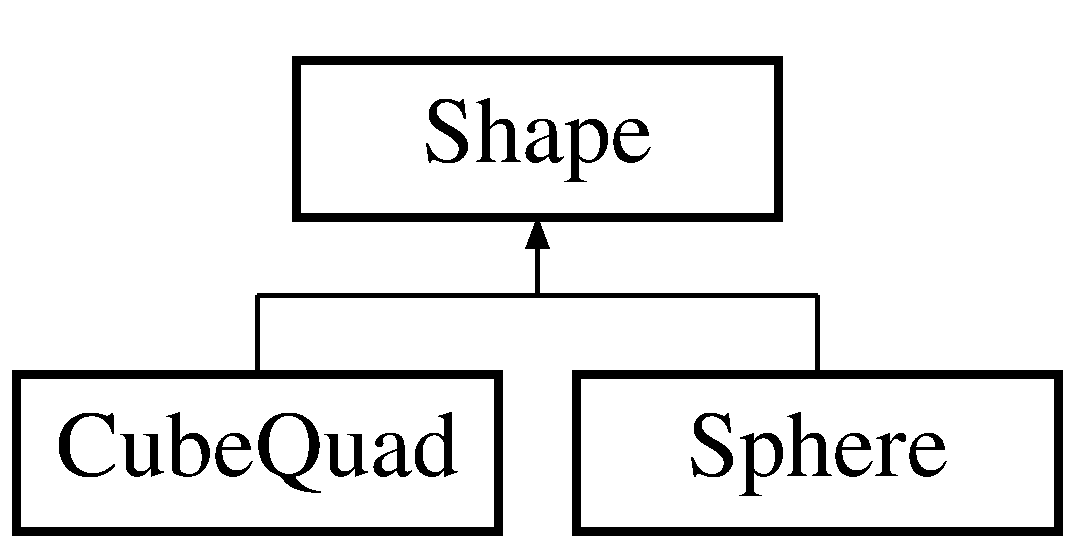
\includegraphics[height=2.000000cm]{class_shape}
\end{center}
\end{figure}
\subsection*{Public Member Functions}
\begin{DoxyCompactItemize}
\item 
\mbox{\Hypertarget{class_shape_ac4d71163e542213ea286344300e16c6f}\label{class_shape_ac4d71163e542213ea286344300e16c6f}} 
virtual \mbox{\hyperlink{class_material}{Material}} {\bfseries get\+Material} () const
\item 
virtual bool \mbox{\hyperlink{class_shape_ab443b81b74cfb1d248d23cc049da7ddd}{is\+\_\+hit}} (\mbox{\hyperlink{class_ray3f}{Ray3f}} \&ray)=0
\begin{DoxyCompactList}\small\item\em Find if there\textquotesingle{}s an intersection between an object and a ray. \end{DoxyCompactList}\item 
virtual \mbox{\hyperlink{class_ray3f}{Ray3f}} \mbox{\hyperlink{class_shape_a7cc30a4c8e9564c51f6ab36554aa5cfc}{reflect}} (\mbox{\hyperlink{class_ray3f}{Ray3f}} ray)=0
\begin{DoxyCompactList}\small\item\em Give the reflection ray of another ray that hit an object. \end{DoxyCompactList}\item 
virtual \mbox{\hyperlink{class_vector3f}{Vector3f}} \mbox{\hyperlink{class_shape_afba80076ff9eb95f7e7c4144e323590f}{get\+Normal}} (\mbox{\hyperlink{class_vector3f}{Vector3f}} position)=0
\begin{DoxyCompactList}\small\item\em Find the normal vector of an object. \end{DoxyCompactList}\item 
virtual double \mbox{\hyperlink{class_shape_aae1d31ff6fb4237397bf11afd07d7e48}{Intersection}} (\mbox{\hyperlink{class_ray3f}{Ray3f}} ray)=0
\begin{DoxyCompactList}\small\item\em Find the intersection position between an object and a ray. \end{DoxyCompactList}\end{DoxyCompactItemize}
\subsection*{Protected Attributes}
\begin{DoxyCompactItemize}
\item 
\mbox{\Hypertarget{class_shape_a233d59f3966db1560b944cc33a4712de}\label{class_shape_a233d59f3966db1560b944cc33a4712de}} 
\mbox{\hyperlink{class_material}{Material}} {\bfseries matter\+\_\+}
\end{DoxyCompactItemize}


\subsection{Member Function Documentation}
\mbox{\Hypertarget{class_shape_afba80076ff9eb95f7e7c4144e323590f}\label{class_shape_afba80076ff9eb95f7e7c4144e323590f}} 
\index{Shape@{Shape}!get\+Normal@{get\+Normal}}
\index{get\+Normal@{get\+Normal}!Shape@{Shape}}
\subsubsection{\texorpdfstring{get\+Normal()}{getNormal()}}
{\footnotesize\ttfamily virtual \mbox{\hyperlink{class_vector3f}{Vector3f}} Shape\+::get\+Normal (\begin{DoxyParamCaption}\item[{\mbox{\hyperlink{class_vector3f}{Vector3f}}}]{position }\end{DoxyParamCaption})\hspace{0.3cm}{\ttfamily [pure virtual]}}



Find the normal vector of an object. 

give the normal vector from a position 
\begin{DoxyParams}{Parameters}
{\em ray} & \mbox{\hyperlink{class_vector3f}{Vector3f}} \\
\hline
\end{DoxyParams}
\begin{DoxyReturn}{Returns}
\mbox{\hyperlink{class_vector3f}{Vector3f}}\+: the normal vector 
\end{DoxyReturn}


Implemented in \mbox{\hyperlink{class_cube_quad_aba1f984ce9580e2e430ace0137a0f249}{Cube\+Quad}}, and \mbox{\hyperlink{class_sphere_a46b57f659960b0862efcb6a7be9f1846}{Sphere}}.

\mbox{\Hypertarget{class_shape_aae1d31ff6fb4237397bf11afd07d7e48}\label{class_shape_aae1d31ff6fb4237397bf11afd07d7e48}} 
\index{Shape@{Shape}!Intersection@{Intersection}}
\index{Intersection@{Intersection}!Shape@{Shape}}
\subsubsection{\texorpdfstring{Intersection()}{Intersection()}}
{\footnotesize\ttfamily virtual double Shape\+::\+Intersection (\begin{DoxyParamCaption}\item[{\mbox{\hyperlink{class_ray3f}{Ray3f}}}]{ray }\end{DoxyParamCaption})\hspace{0.3cm}{\ttfamily [pure virtual]}}



Find the intersection position between an object and a ray. 

give the intersection position if there\textquotesingle{}s an intersection return -\/1 if there\textquotesingle{}s no intersection 
\begin{DoxyParams}{Parameters}
{\em ray} & \mbox{\hyperlink{class_ray3f}{Ray3f}} \\
\hline
\end{DoxyParams}
\begin{DoxyReturn}{Returns}
double the distance from our ray origin to the point of intersection return -\/1 if there\textquotesingle{}s no intersection 
\end{DoxyReturn}


Implemented in \mbox{\hyperlink{class_cube_quad_a3b51f8216f2ba340174edb542af33c0a}{Cube\+Quad}}, and \mbox{\hyperlink{class_sphere_af9c784cb35851974251e1585e3717dd9}{Sphere}}.

\mbox{\Hypertarget{class_shape_ab443b81b74cfb1d248d23cc049da7ddd}\label{class_shape_ab443b81b74cfb1d248d23cc049da7ddd}} 
\index{Shape@{Shape}!is\+\_\+hit@{is\+\_\+hit}}
\index{is\+\_\+hit@{is\+\_\+hit}!Shape@{Shape}}
\subsubsection{\texorpdfstring{is\+\_\+hit()}{is\_hit()}}
{\footnotesize\ttfamily virtual bool Shape\+::is\+\_\+hit (\begin{DoxyParamCaption}\item[{\mbox{\hyperlink{class_ray3f}{Ray3f}} \&}]{ray }\end{DoxyParamCaption})\hspace{0.3cm}{\ttfamily [pure virtual]}}



Find if there\textquotesingle{}s an intersection between an object and a ray. 

Find if there\textquotesingle{}s an intersection between an object and a ray and give intersect of ray3f\+: the value of the distance from ray\textquotesingle{}s origin to the point of intersection 
\begin{DoxyParams}{Parameters}
{\em ray} & \mbox{\hyperlink{class_ray3f}{Ray3f}} \\
\hline
\end{DoxyParams}
\begin{DoxyReturn}{Returns}
bool true if we have intersection 
\end{DoxyReturn}


Implemented in \mbox{\hyperlink{class_cube_quad_a8d55228ceeed7ce319bc6d8fe8f6b67f}{Cube\+Quad}}, and \mbox{\hyperlink{class_sphere_a29e5c6f306c166c59b5d462205177f27}{Sphere}}.

\mbox{\Hypertarget{class_shape_a7cc30a4c8e9564c51f6ab36554aa5cfc}\label{class_shape_a7cc30a4c8e9564c51f6ab36554aa5cfc}} 
\index{Shape@{Shape}!reflect@{reflect}}
\index{reflect@{reflect}!Shape@{Shape}}
\subsubsection{\texorpdfstring{reflect()}{reflect()}}
{\footnotesize\ttfamily virtual \mbox{\hyperlink{class_ray3f}{Ray3f}} Shape\+::reflect (\begin{DoxyParamCaption}\item[{\mbox{\hyperlink{class_ray3f}{Ray3f}}}]{ray }\end{DoxyParamCaption})\hspace{0.3cm}{\ttfamily [pure virtual]}}



Give the reflection ray of another ray that hit an object. 

Give the reflection ray from the intersection position 
\begin{DoxyParams}{Parameters}
{\em ray} & \mbox{\hyperlink{class_ray3f}{Ray3f}} \\
\hline
\end{DoxyParams}
\begin{DoxyReturn}{Returns}
\mbox{\hyperlink{class_ray3f}{Ray3f}} \+: the reflected ray 
\end{DoxyReturn}


Implemented in \mbox{\hyperlink{class_cube_quad_a18ef5943f0cfd8b9b72950211691314a}{Cube\+Quad}}, and \mbox{\hyperlink{class_sphere_a4ba50719ce557c0ff9a85333d0524bad}{Sphere}}.



The documentation for this class was generated from the following file\+:\begin{DoxyCompactItemize}
\item 
Shape.\+h\end{DoxyCompactItemize}

\hypertarget{class_sphere}{}\section{Sphere Class Reference}
\label{class_sphere}\index{Sphere@{Sphere}}
Inheritance diagram for Sphere\+:\begin{figure}[H]
\begin{center}
\leavevmode
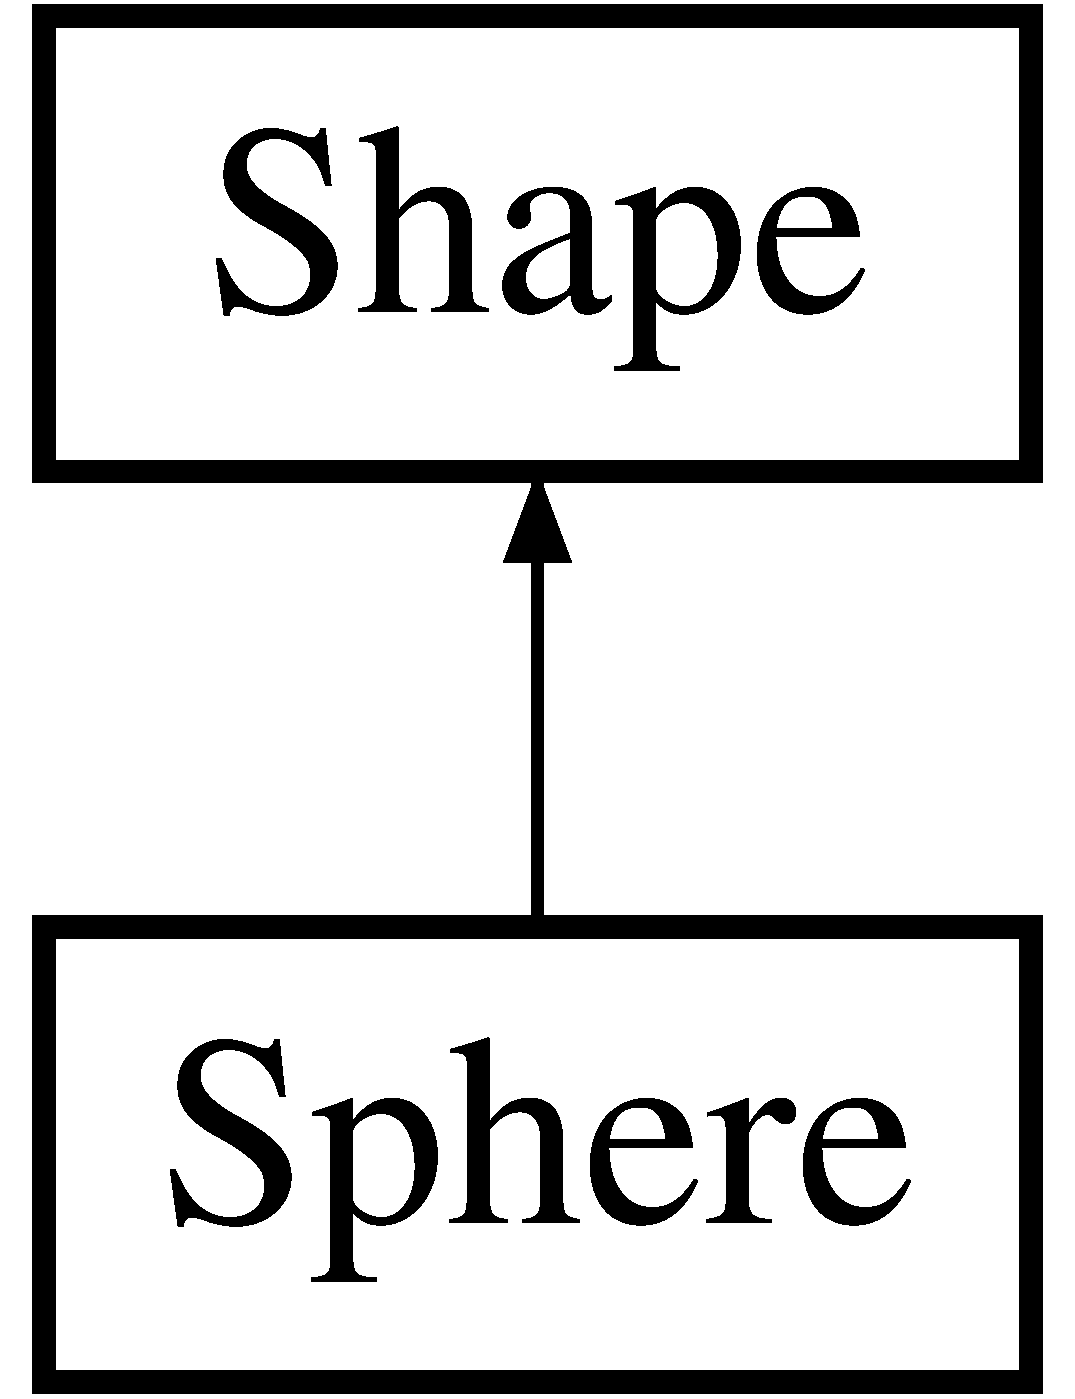
\includegraphics[height=2.000000cm]{class_sphere}
\end{center}
\end{figure}
\subsection*{Public Member Functions}
\begin{DoxyCompactItemize}
\item 
\mbox{\Hypertarget{class_sphere_a9c65eef465ec94ededb06398a8be246c}\label{class_sphere_a9c65eef465ec94ededb06398a8be246c}} 
{\bfseries Sphere} (\mbox{\hyperlink{class_material}{Material}} m, \mbox{\hyperlink{class_vector3f}{Vector3f}} origin, float radius)
\item 
\mbox{\Hypertarget{class_sphere_abe994d42b65ae2f23efed35b994e3434}\label{class_sphere_abe994d42b65ae2f23efed35b994e3434}} 
\mbox{\hyperlink{class_vector3f}{Vector3f}} {\bfseries get\+Origin} () const
\item 
\mbox{\Hypertarget{class_sphere_a925a4eccca10735eb3f9ec03ad87abf1}\label{class_sphere_a925a4eccca10735eb3f9ec03ad87abf1}} 
float {\bfseries get\+Radius} () const
\item 
virtual bool \mbox{\hyperlink{class_sphere_a29e5c6f306c166c59b5d462205177f27}{is\+\_\+hit}} (\mbox{\hyperlink{class_ray3f}{Ray3f}} \&ray)
\begin{DoxyCompactList}\small\item\em Find if there\textquotesingle{}s an intersection between an object and a ray. \end{DoxyCompactList}\item 
virtual \mbox{\hyperlink{class_ray3f}{Ray3f}} \mbox{\hyperlink{class_sphere_a4ba50719ce557c0ff9a85333d0524bad}{reflect}} (\mbox{\hyperlink{class_ray3f}{Ray3f}} ray)
\begin{DoxyCompactList}\small\item\em Give the reflection ray of another ray that hit an object. \end{DoxyCompactList}\item 
virtual double \mbox{\hyperlink{class_sphere_af9c784cb35851974251e1585e3717dd9}{Intersection}} (\mbox{\hyperlink{class_ray3f}{Ray3f}} ray)
\begin{DoxyCompactList}\small\item\em Find the intersection position between an object and a ray. \end{DoxyCompactList}\item 
virtual \mbox{\hyperlink{class_vector3f}{Vector3f}} \mbox{\hyperlink{class_sphere_a46b57f659960b0862efcb6a7be9f1846}{get\+Normal}} (\mbox{\hyperlink{class_vector3f}{Vector3f}} position)
\begin{DoxyCompactList}\small\item\em Find the normal vector of an object. \end{DoxyCompactList}\end{DoxyCompactItemize}
\subsection*{Additional Inherited Members}


\subsection{Member Function Documentation}
\mbox{\Hypertarget{class_sphere_a46b57f659960b0862efcb6a7be9f1846}\label{class_sphere_a46b57f659960b0862efcb6a7be9f1846}} 
\index{Sphere@{Sphere}!get\+Normal@{get\+Normal}}
\index{get\+Normal@{get\+Normal}!Sphere@{Sphere}}
\subsubsection{\texorpdfstring{get\+Normal()}{getNormal()}}
{\footnotesize\ttfamily virtual \mbox{\hyperlink{class_vector3f}{Vector3f}} Sphere\+::get\+Normal (\begin{DoxyParamCaption}\item[{\mbox{\hyperlink{class_vector3f}{Vector3f}}}]{position }\end{DoxyParamCaption})\hspace{0.3cm}{\ttfamily [inline]}, {\ttfamily [virtual]}}



Find the normal vector of an object. 

give the normal vector from a position 
\begin{DoxyParams}{Parameters}
{\em ray} & \mbox{\hyperlink{class_vector3f}{Vector3f}} \\
\hline
\end{DoxyParams}
\begin{DoxyReturn}{Returns}
\mbox{\hyperlink{class_vector3f}{Vector3f}}\+: the normal vector 
\end{DoxyReturn}


Implements \mbox{\hyperlink{class_shape_afba80076ff9eb95f7e7c4144e323590f}{Shape}}.

\mbox{\Hypertarget{class_sphere_af9c784cb35851974251e1585e3717dd9}\label{class_sphere_af9c784cb35851974251e1585e3717dd9}} 
\index{Sphere@{Sphere}!Intersection@{Intersection}}
\index{Intersection@{Intersection}!Sphere@{Sphere}}
\subsubsection{\texorpdfstring{Intersection()}{Intersection()}}
{\footnotesize\ttfamily double Sphere\+::\+Intersection (\begin{DoxyParamCaption}\item[{\mbox{\hyperlink{class_ray3f}{Ray3f}}}]{ray }\end{DoxyParamCaption})\hspace{0.3cm}{\ttfamily [virtual]}}



Find the intersection position between an object and a ray. 

give the intersection position if there\textquotesingle{}s an intersection return -\/1 if there\textquotesingle{}s no intersection 
\begin{DoxyParams}{Parameters}
{\em ray} & \mbox{\hyperlink{class_ray3f}{Ray3f}} \\
\hline
\end{DoxyParams}
\begin{DoxyReturn}{Returns}
double the distance from our ray origin to the point of intersection return -\/1 if there\textquotesingle{}s no intersection 
\end{DoxyReturn}


Implements \mbox{\hyperlink{class_shape_aae1d31ff6fb4237397bf11afd07d7e48}{Shape}}.

\mbox{\Hypertarget{class_sphere_a29e5c6f306c166c59b5d462205177f27}\label{class_sphere_a29e5c6f306c166c59b5d462205177f27}} 
\index{Sphere@{Sphere}!is\+\_\+hit@{is\+\_\+hit}}
\index{is\+\_\+hit@{is\+\_\+hit}!Sphere@{Sphere}}
\subsubsection{\texorpdfstring{is\+\_\+hit()}{is\_hit()}}
{\footnotesize\ttfamily bool Sphere\+::is\+\_\+hit (\begin{DoxyParamCaption}\item[{\mbox{\hyperlink{class_ray3f}{Ray3f}} \&}]{ray }\end{DoxyParamCaption})\hspace{0.3cm}{\ttfamily [virtual]}}



Find if there\textquotesingle{}s an intersection between an object and a ray. 

Find if there\textquotesingle{}s an intersection between an object and a ray and give intersect of ray3f\+: the value of the distance from ray\textquotesingle{}s origin to the point of intersection 
\begin{DoxyParams}{Parameters}
{\em ray} & \mbox{\hyperlink{class_ray3f}{Ray3f}} \\
\hline
\end{DoxyParams}
\begin{DoxyReturn}{Returns}
bool true if we have intersection 
\end{DoxyReturn}


Implements \mbox{\hyperlink{class_shape_ab443b81b74cfb1d248d23cc049da7ddd}{Shape}}.

\mbox{\Hypertarget{class_sphere_a4ba50719ce557c0ff9a85333d0524bad}\label{class_sphere_a4ba50719ce557c0ff9a85333d0524bad}} 
\index{Sphere@{Sphere}!reflect@{reflect}}
\index{reflect@{reflect}!Sphere@{Sphere}}
\subsubsection{\texorpdfstring{reflect()}{reflect()}}
{\footnotesize\ttfamily \mbox{\hyperlink{class_ray3f}{Ray3f}} Sphere\+::reflect (\begin{DoxyParamCaption}\item[{\mbox{\hyperlink{class_ray3f}{Ray3f}}}]{ray }\end{DoxyParamCaption})\hspace{0.3cm}{\ttfamily [virtual]}}



Give the reflection ray of another ray that hit an object. 

Give the reflection ray from the intersection position 
\begin{DoxyParams}{Parameters}
{\em ray} & \mbox{\hyperlink{class_ray3f}{Ray3f}} \\
\hline
\end{DoxyParams}
\begin{DoxyReturn}{Returns}
{\itshape \mbox{\hyperlink{class_ray3f}{Ray3f}}} \+: the reflected ray 
\end{DoxyReturn}


Implements \mbox{\hyperlink{class_shape_a7cc30a4c8e9564c51f6ab36554aa5cfc}{Shape}}.



The documentation for this class was generated from the following files\+:\begin{DoxyCompactItemize}
\item 
Sphere.\+h\item 
Sphere.\+cpp\end{DoxyCompactItemize}

\hypertarget{class_vector3f}{}\section{Vector3f Class Reference}
\label{class_vector3f}\index{Vector3f@{Vector3f}}
\subsection*{Public Member Functions}
\begin{DoxyCompactItemize}
\item 
\mbox{\Hypertarget{class_vector3f_a71033a308401bb8950d846a012d13da8}\label{class_vector3f_a71033a308401bb8950d846a012d13da8}} 
{\bfseries Vector3f} (float x, float y, float z)
\item 
\mbox{\Hypertarget{class_vector3f_ae1ae69e00043d02ebd7c7e4a24dde877}\label{class_vector3f_ae1ae69e00043d02ebd7c7e4a24dde877}} 
{\bfseries Vector3f} (const \mbox{\hyperlink{class_vector3f}{Vector3f}} \&v)
\item 
\mbox{\Hypertarget{class_vector3f_a76759eb4a7879906441ed9ad7385e4c3}\label{class_vector3f_a76759eb4a7879906441ed9ad7385e4c3}} 
float {\bfseries getX} () const
\item 
\mbox{\Hypertarget{class_vector3f_a2cf82f229b7d7d5398d7c9fd453a0fbc}\label{class_vector3f_a2cf82f229b7d7d5398d7c9fd453a0fbc}} 
float {\bfseries getY} () const
\item 
\mbox{\Hypertarget{class_vector3f_a0a87d639c7172d1c9eea7fac74f5e6ae}\label{class_vector3f_a0a87d639c7172d1c9eea7fac74f5e6ae}} 
float {\bfseries getZ} () const
\item 
\mbox{\Hypertarget{class_vector3f_a3999baa8fa2c761253362f7e5f68bfec}\label{class_vector3f_a3999baa8fa2c761253362f7e5f68bfec}} 
void {\bfseries setX} (float x)
\item 
\mbox{\Hypertarget{class_vector3f_a533d6931dc15f0f0e66b094debeaf4ce}\label{class_vector3f_a533d6931dc15f0f0e66b094debeaf4ce}} 
void {\bfseries setY} (float y)
\item 
\mbox{\Hypertarget{class_vector3f_a0cb5d2450424090a599f0e429f8f3a34}\label{class_vector3f_a0cb5d2450424090a599f0e429f8f3a34}} 
void {\bfseries setZ} (float z)
\item 
\mbox{\Hypertarget{class_vector3f_a6081a4bd906d2f0eda56ffb6a35d8218}\label{class_vector3f_a6081a4bd906d2f0eda56ffb6a35d8218}} 
float {\bfseries length2} () const
\item 
\mbox{\Hypertarget{class_vector3f_a92cc3ac93ffeb9d379398975d2232881}\label{class_vector3f_a92cc3ac93ffeb9d379398975d2232881}} 
float {\bfseries length} () const
\item 
\mbox{\Hypertarget{class_vector3f_af86f3422d11cfb5e56bdada4b4bc68cc}\label{class_vector3f_af86f3422d11cfb5e56bdada4b4bc68cc}} 
\mbox{\hyperlink{class_vector3f}{Vector3f}} {\bfseries normalize} ()
\item 
\mbox{\Hypertarget{class_vector3f_a4ddb5ce190456e116f0715fb72ff9cce}\label{class_vector3f_a4ddb5ce190456e116f0715fb72ff9cce}} 
float {\bfseries dot} (const \mbox{\hyperlink{class_vector3f}{Vector3f}} \&v) const
\item 
\mbox{\Hypertarget{class_vector3f_aeca2c55dc36f17ef3b602f714ae180cc}\label{class_vector3f_aeca2c55dc36f17ef3b602f714ae180cc}} 
\mbox{\hyperlink{class_vector3f}{Vector3f}} {\bfseries cross\+Product} (\mbox{\hyperlink{class_vector3f}{Vector3f}} v)
\item 
\mbox{\Hypertarget{class_vector3f_a914d927662bb2494bd5f5dcc0df57cfa}\label{class_vector3f_a914d927662bb2494bd5f5dcc0df57cfa}} 
\mbox{\hyperlink{class_vector3f}{Vector3f}} {\bfseries operator+} (const \mbox{\hyperlink{class_vector3f}{Vector3f}} \&v) const
\item 
\mbox{\Hypertarget{class_vector3f_a2f5f71db2b48c61bce44e5932cea5125}\label{class_vector3f_a2f5f71db2b48c61bce44e5932cea5125}} 
\mbox{\hyperlink{class_vector3f}{Vector3f}} {\bfseries operator-\/} (const \mbox{\hyperlink{class_vector3f}{Vector3f}} \&v) const
\item 
\mbox{\Hypertarget{class_vector3f_a64b8be69e77e9af068e6c0cae71b51f2}\label{class_vector3f_a64b8be69e77e9af068e6c0cae71b51f2}} 
\mbox{\hyperlink{class_vector3f}{Vector3f}} {\bfseries operator-\/} () const
\item 
\mbox{\Hypertarget{class_vector3f_a9cb61c27e0ca0fe0ab9f985fb2fe2b22}\label{class_vector3f_a9cb61c27e0ca0fe0ab9f985fb2fe2b22}} 
\mbox{\hyperlink{class_vector3f}{Vector3f}} {\bfseries operator$\ast$} (const \mbox{\hyperlink{class_vector3f}{Vector3f}} \&v) const
\item 
\mbox{\Hypertarget{class_vector3f_a3146962450ac1e2b990741598f4dc9fc}\label{class_vector3f_a3146962450ac1e2b990741598f4dc9fc}} 
\mbox{\hyperlink{class_vector3f}{Vector3f}} {\bfseries operator$\ast$} (float f) const
\end{DoxyCompactItemize}
\subsection*{Friends}
\begin{DoxyCompactItemize}
\item 
\mbox{\Hypertarget{class_vector3f_aa1e7b077412a7dda14250db481497613}\label{class_vector3f_aa1e7b077412a7dda14250db481497613}} 
\mbox{\hyperlink{class_vector3f}{Vector3f}} {\bfseries operator$\ast$} (float val, const \mbox{\hyperlink{class_vector3f}{Vector3f}} \&v)
\item 
\mbox{\Hypertarget{class_vector3f_ae11044c18269c8fef450ab53e6cc6290}\label{class_vector3f_ae11044c18269c8fef450ab53e6cc6290}} 
std\+::ostream \& {\bfseries operator$<$$<$} (std\+::ostream \&std, const \mbox{\hyperlink{class_vector3f}{Vector3f}} \&v)
\end{DoxyCompactItemize}


The documentation for this class was generated from the following files\+:\begin{DoxyCompactItemize}
\item 
Vector3f.\+h\item 
Vector3f.\+cpp\end{DoxyCompactItemize}

%--- End generated contents ---

% Index
\backmatter
\newpage
\phantomsection
\clearemptydoublepage
\addcontentsline{toc}{chapter}{Index}
\printindex

\end{document}
